\documentclass[11pt,a4paper]{article}
\usepackage[utf8]{inputenc}
\usepackage[spanish]{babel}
\usepackage{amsmath, amssymb, amsthm, amsfonts}
\usepackage{graphicx}
\usepackage{geometry}
\usepackage{float}
\usepackage{bm}
\usepackage{hyperref}
\hypersetup{
    colorlinks=true,
    linktoc=all,
    linkcolor=blue,
}
\usepackage{multirow}
\usepackage{comment}
\usepackage{cleveref}
\usepackage{background}
\usepackage{tikz}

\backgroundsetup{
  scale=1,
  color=black,
  opacity=0.15,
  angle=0,
  position=current page.south west,
  vshift=4cm,
  hshift=1cm,
  contents={
\includegraphics[width=\textwidth]{LogoUGR.png}}
}

\geometry{margin=2.5cm}
\title{Electrónica Física\\
titulo ingenioso}
\author{Sharan Haresh Belani, Juan Montaraz Gómez, María Ramos Calderón\\ \&
Nuria Touriño Verano}

\begin{document}

\maketitle

\section{Introducción}
En esta práctica analizamos el transporte cuántico utilizando la herramienta \texttt{Piece-Wise Constant Potential Barrier Tool} de nanoHUB \cite{nano}, que destaca por su versatilidad para simular heteroestructuras de distintas características. En este trabajo nos centraremos en variar el \textbf{número} de barreras (y, consecuentemente, de pozos) en el simulador para emular una red de micelio. En esta analogía, cada pozo cuántico representa una unidad celular fúngica, y cada barrera de potencial representa la interconexión entre ellas (septo). La primera y la última célula del dispositivo se consideran acopladas directamente a los contactos del sistema.

Para dotar a la simulación de sentido físico, hemos empleado parámetros típicos de heteroestructuras semiconductoras, fijando una masa efectiva de $m^* = 0.067$ (la del GaAs), una anchura de pozo de $5\text{ nm}$, y barreras de $2\text{ nm}$ con una altura de potencial de $0.4\text{ eV}$. El objetivo principal es estudiar la evolución de la transmitancia al variar la longitud de la cadena desde $N=2$ hasta $N=200$ barreras, observando cómo la concatenación de estados discretos da lugar a la formación de una banda de conducción macroscópica. 

Finalmente, el trabajo evalúa la robustez de este canal de transporte analizando la \textit{frustración del sistema} ante dos patologías o perturbaciones biológicas localizadas en el elemento central de una cadena fija de 5 barreras: la hipertrofia dimensional de una célula (variación del ancho del pozo) y la calcificación o degradación de una interconexión celular (variación del ancho de la barrera).

\section{Resultados}
A continuación, se presentan los coeficientes de transmisión frente a la energía de los electrones incidentes. Todos los resultados han sido procesados y graficados mediante rutinas propias en Python a partir de los datos numéricos exportados del simulador.

En primer lugar, se estudia el régimen de cadenas cortas (de 2 a 5 barreras). La Figura \ref{fig:Junto} muestra la comparativa directa, donde se aprecia el desdoblamiento de los niveles de energía resonantes al aumentar el número de pozos acoplados. La Figura \ref{fig:Separado} desglosa este fenómeno, sombreando las regiones donde la probabilidad de transmisión supera el 50\%, evidenciando el inicio de la formación de minibandas.

\begin{figure}[H]
  \centering
  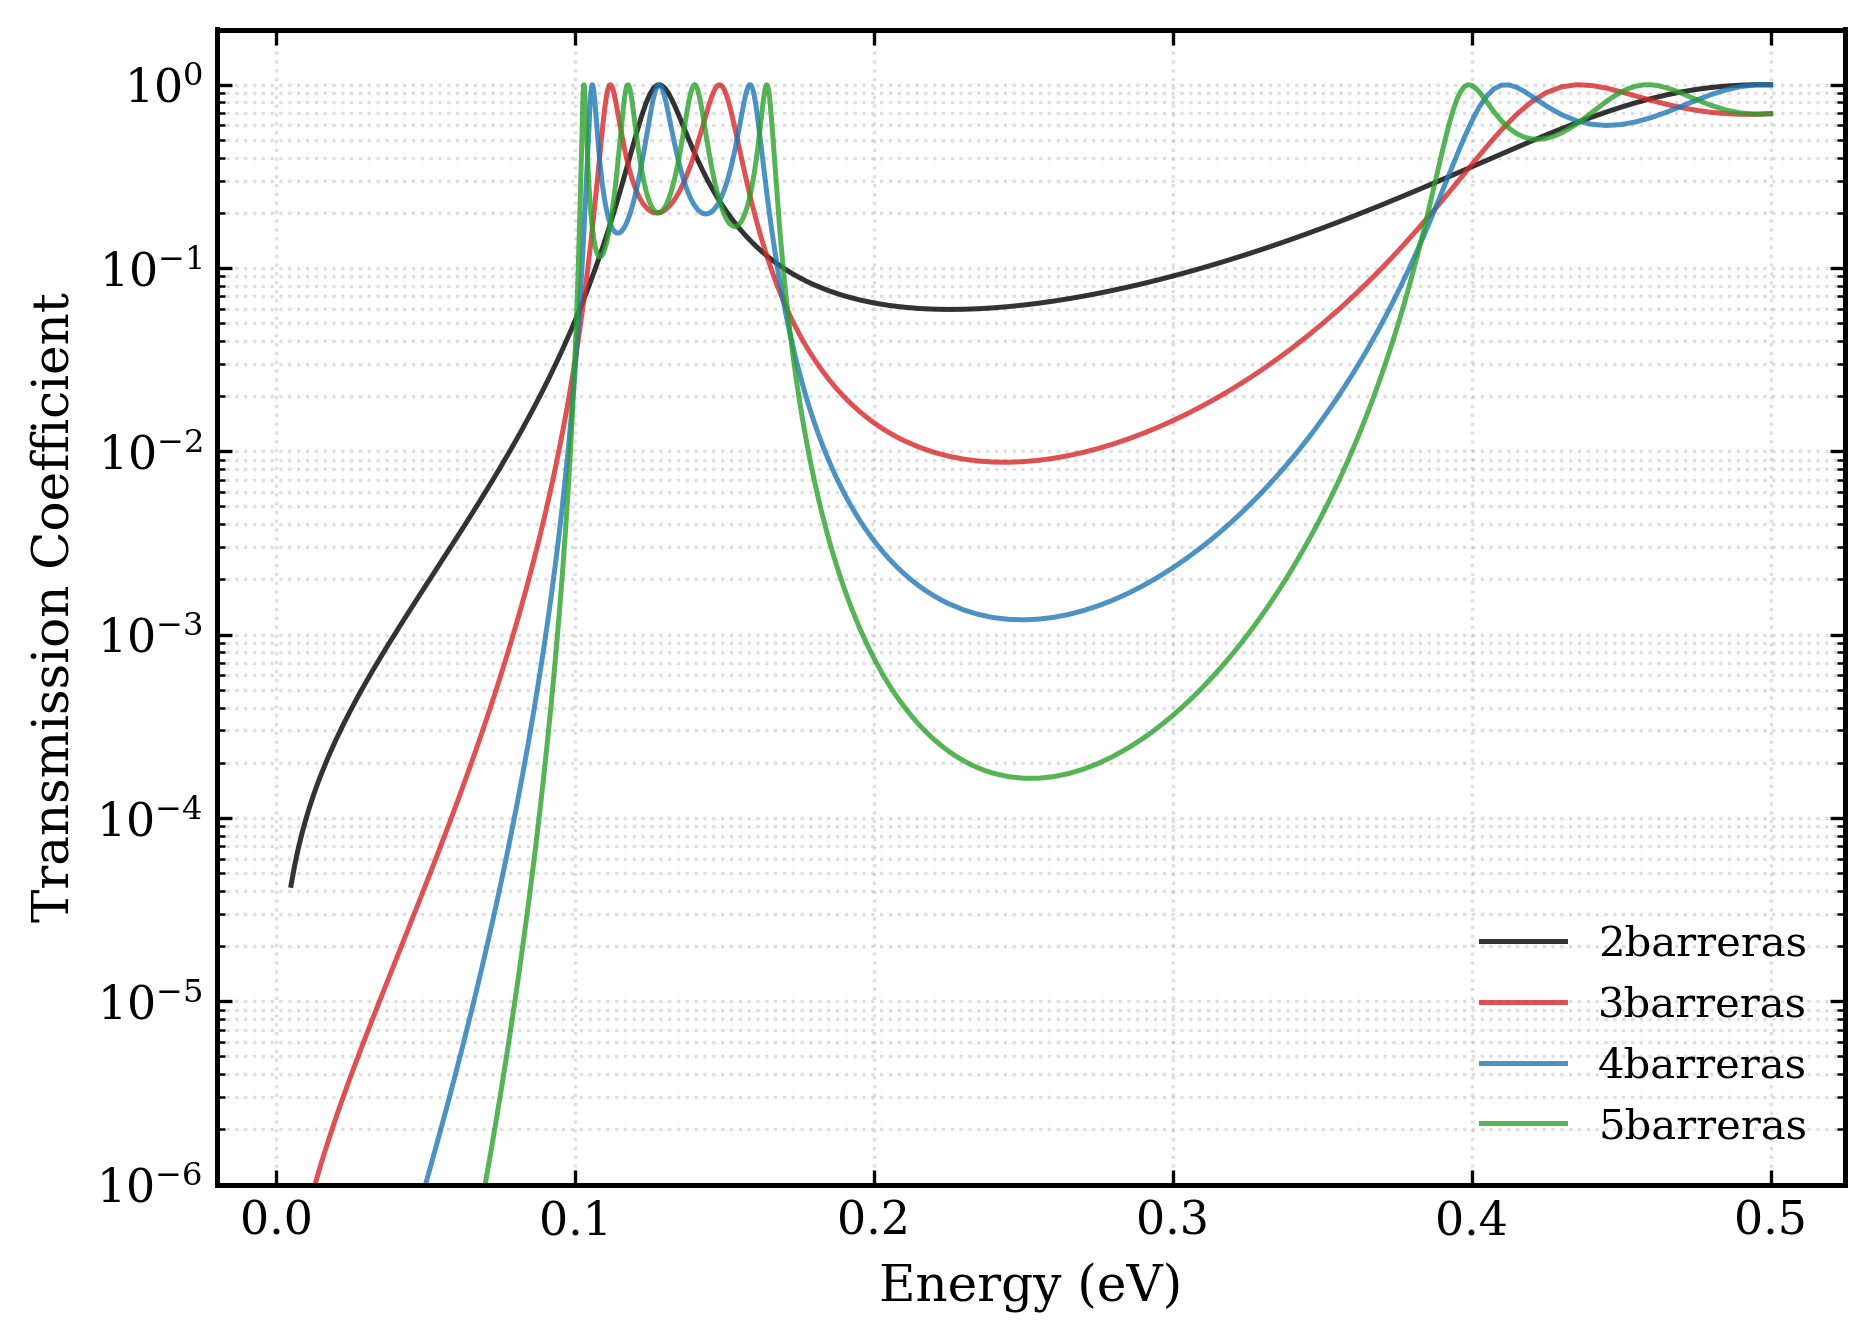
\includegraphics[width=1.0\linewidth]{Junto.png}
  \caption{Coeficientes de Transmisión para $N=2$, $3$, $4$ y $5$ barreras solapadas para ver el canal de transmisión.}
  \label{fig:Junto}
\end{figure}

\begin{figure}[H]
  \centering
  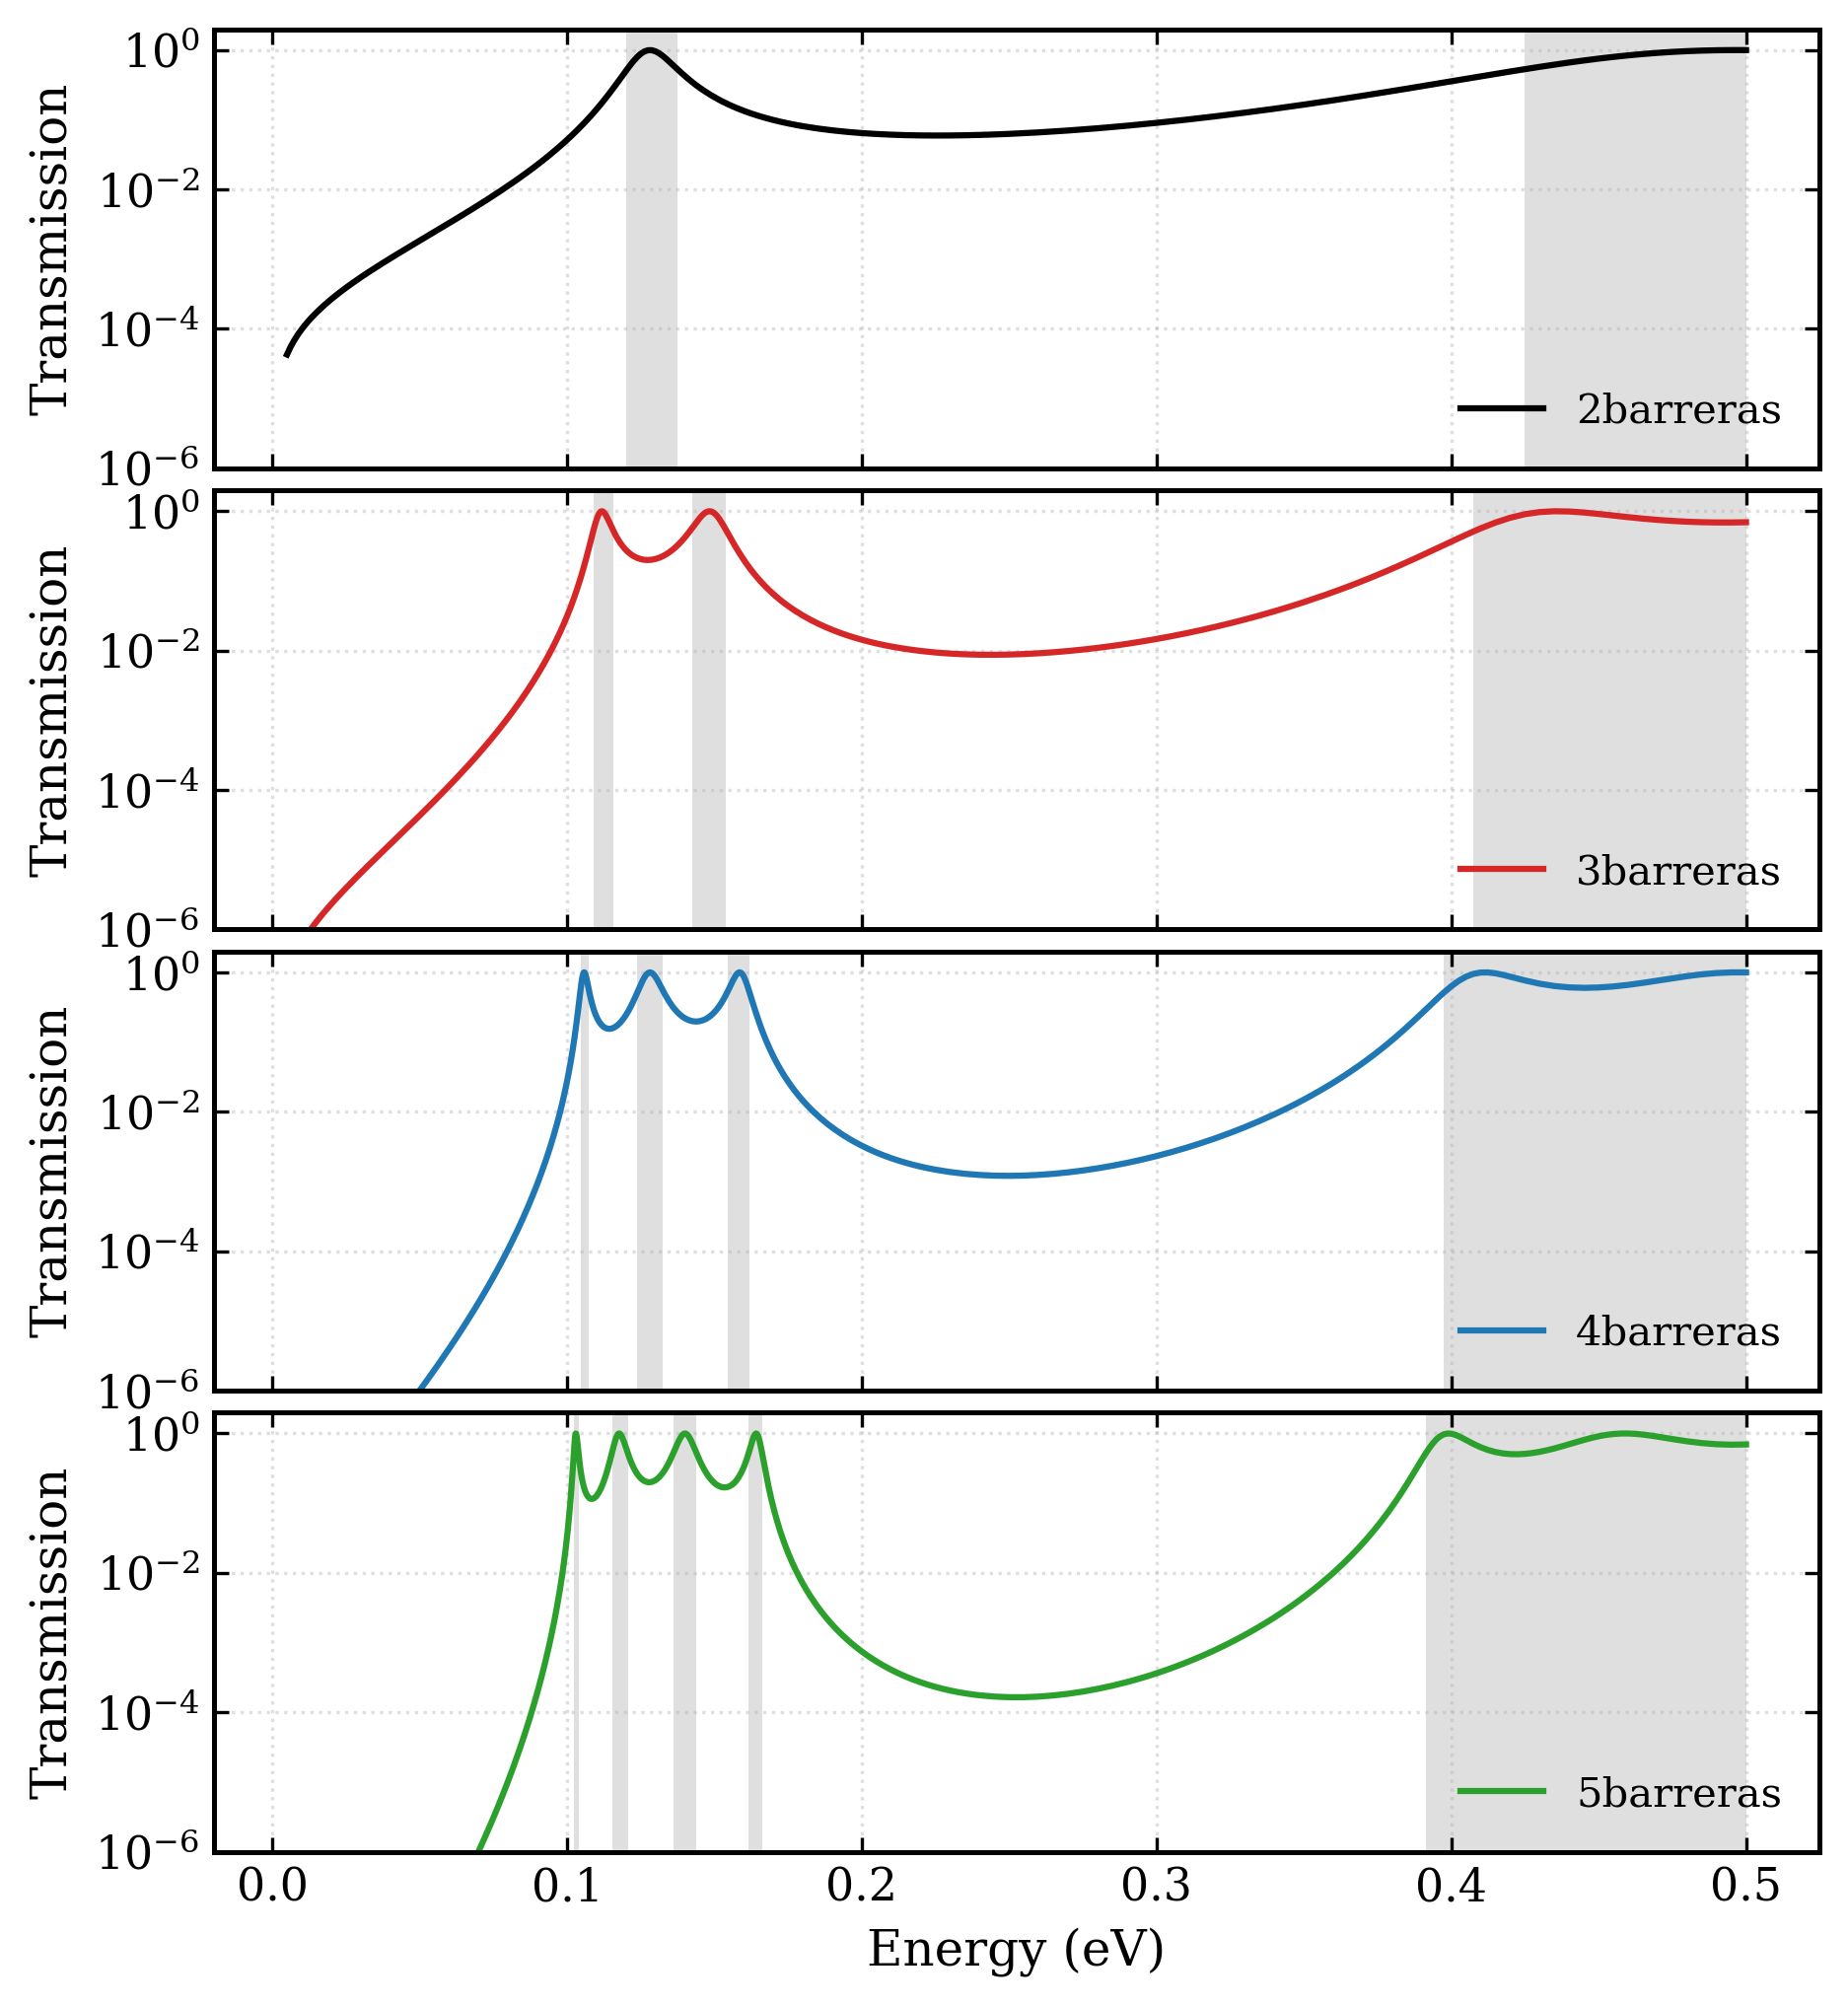
\includegraphics[width=1.0 \linewidth]{Separado.png}
  \caption{Coeficientes de Transmisión para $N=2$, $3$, $4$ y $5$ barreras, destacando zonas de alta transmitancia.}
  \label{fig:Separado}
\end{figure}

Posteriormente, extendemos el análisis al régimen macroscópico (de 8 a 200 barreras), asimilable a un filamento de micelio consolidado. La Figura \ref{fig:Junto_N} ilustra cómo los picos discretos se fusionan definitivamente en una banda continua. Finalmente, la Figura \ref{fig:Separado_N} muestra de forma individual cómo los bordes de esta banda de transmisión se vuelven completamente verticales y estables en cadenas largas, permitiendo una transmisión cercana a 1 en un rango continuo de energías.

\begin{figure}[H]
  \centering
  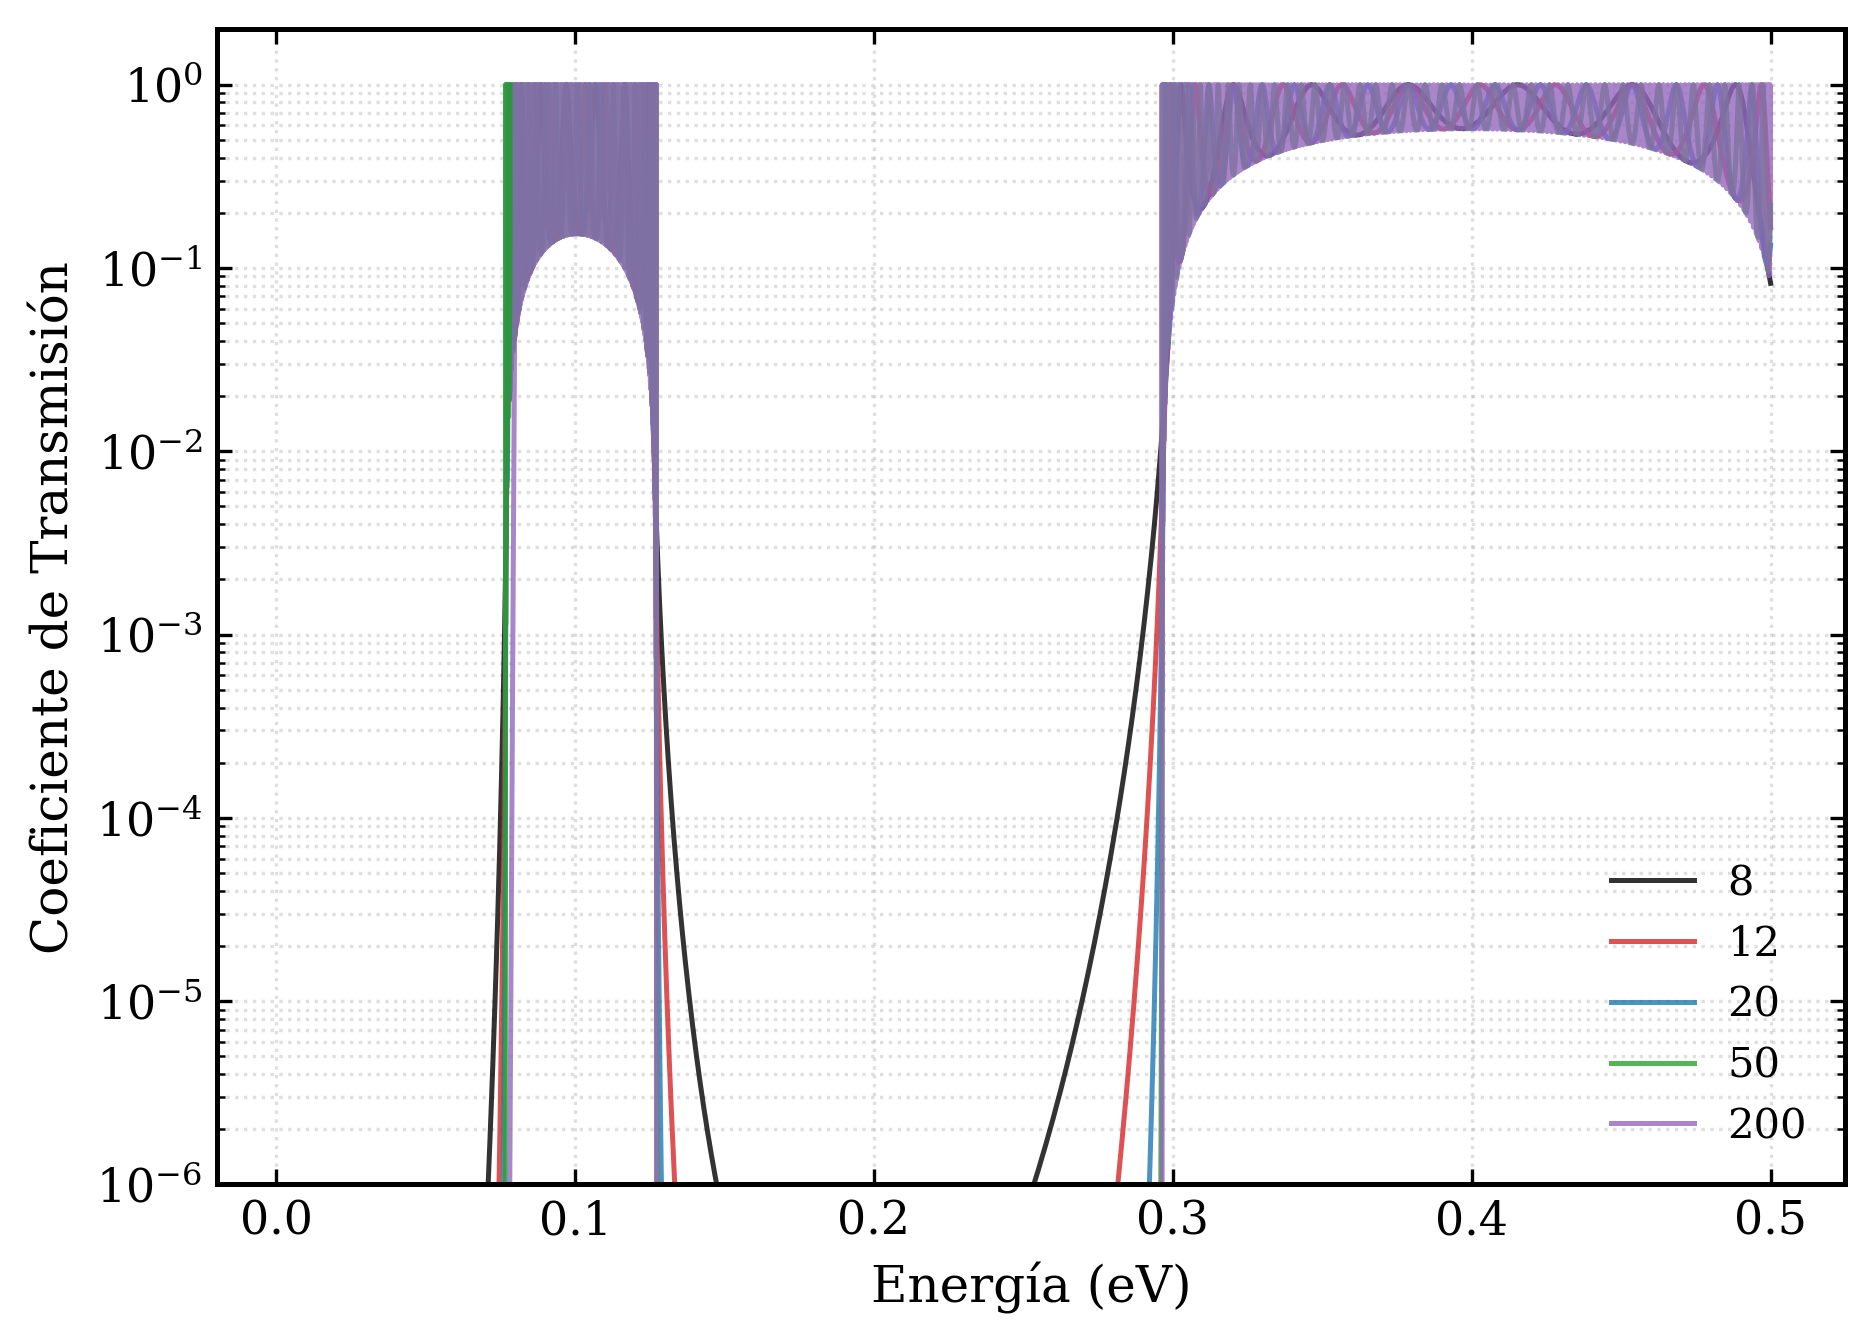
\includegraphics[width=1.0 \linewidth]{Junto_N.png}
  \caption{Coeficientes de Transmisión para $N=8$, $12$, $20$, $50$ y $200$ barreras solapadas para ver el canal de transmisión.}
  \label{fig:Junto_N}
\end{figure}

\begin{figure}[H]
  \centering
  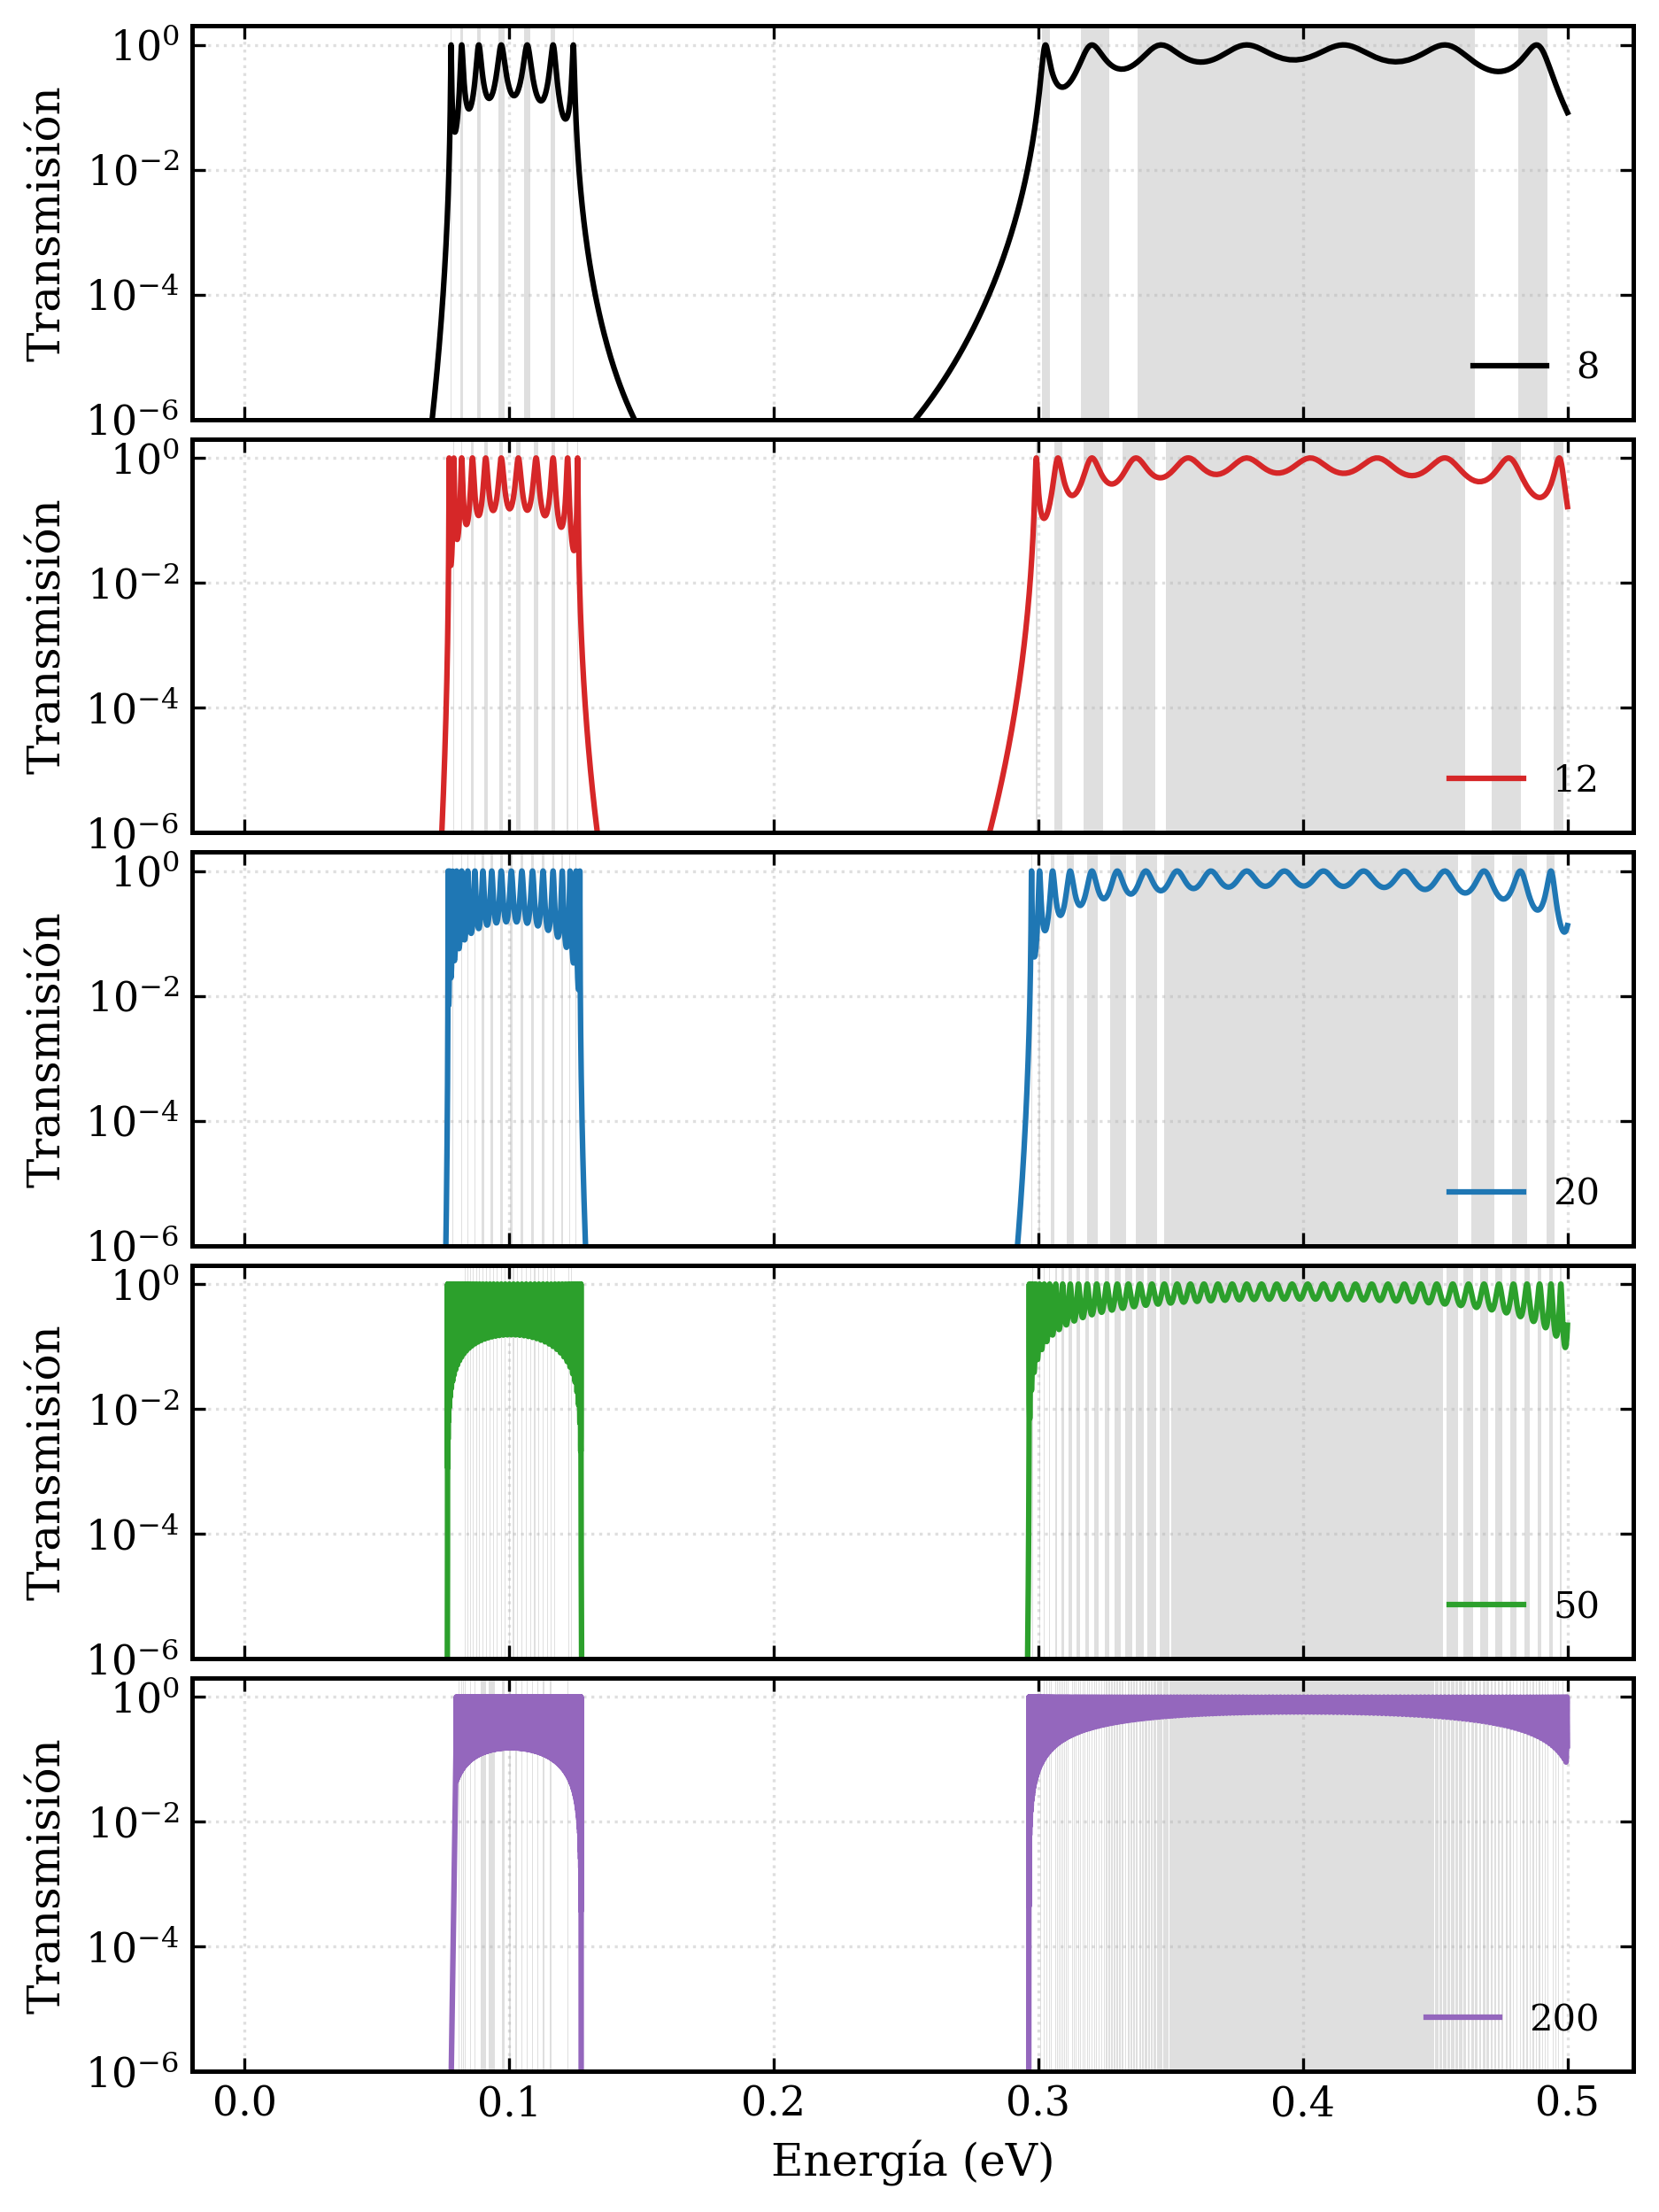
\includegraphics[width=1.0\linewidth]{Separado_N (1).png}
  \caption{Coeficientes de Transmisión para $N=8$, $12$, $20$, $50$ y $200$ barreras, destacando zonas de alta transmitancia.}
  \label{fig:Separado_N}
\end{figure}

% Vemso que la transmisión se puede frustrar de varias maneras, de forma que eso puede ayudar en la historia
% Manera 1: el hongo se vuelve enorme, manera 2: la interconexión entre hongos se bloquea.


Por último, se analiza la respuesta del dispositivo fúngico ante perturbaciones estructurales localizadas utilizando como base el modelo simétrico de 5 barreras (4 pozos). Se evalúan de forma independiente dos escenarios críticos de frustración de la transmisión.

El primer escenario modela una alteración morfológica en la célula fúngica central, incrementando su longitud de $6\text{ nm}$ a $10\text{ nm}$ (estado asimilable a una célula dañada o hipertrofiada). Como se observa en la Figura \ref{fig:Interfase_Rota}, este cambio altera la simetría de la heteroestructura y rompe las condiciones de efecto túnel resonante global. Al ensancharse el pozo central, sus autovalores de energía permitidos se desplazan hacia valores inferiores ($E_n \propto 1/L^2$), desalineándose de los niveles cuánticos de los pozos adyacentes. Como consecuencia directa, el coeficiente de transmisión en la zona de la minibanda (alrededor de $0.35\text{ eV}$) experimenta una drástica caída, colapsando el canal desde un valor ideal de 1 hasta aproximadamente 0.51.

\begin{figure}[H]
  \centering
  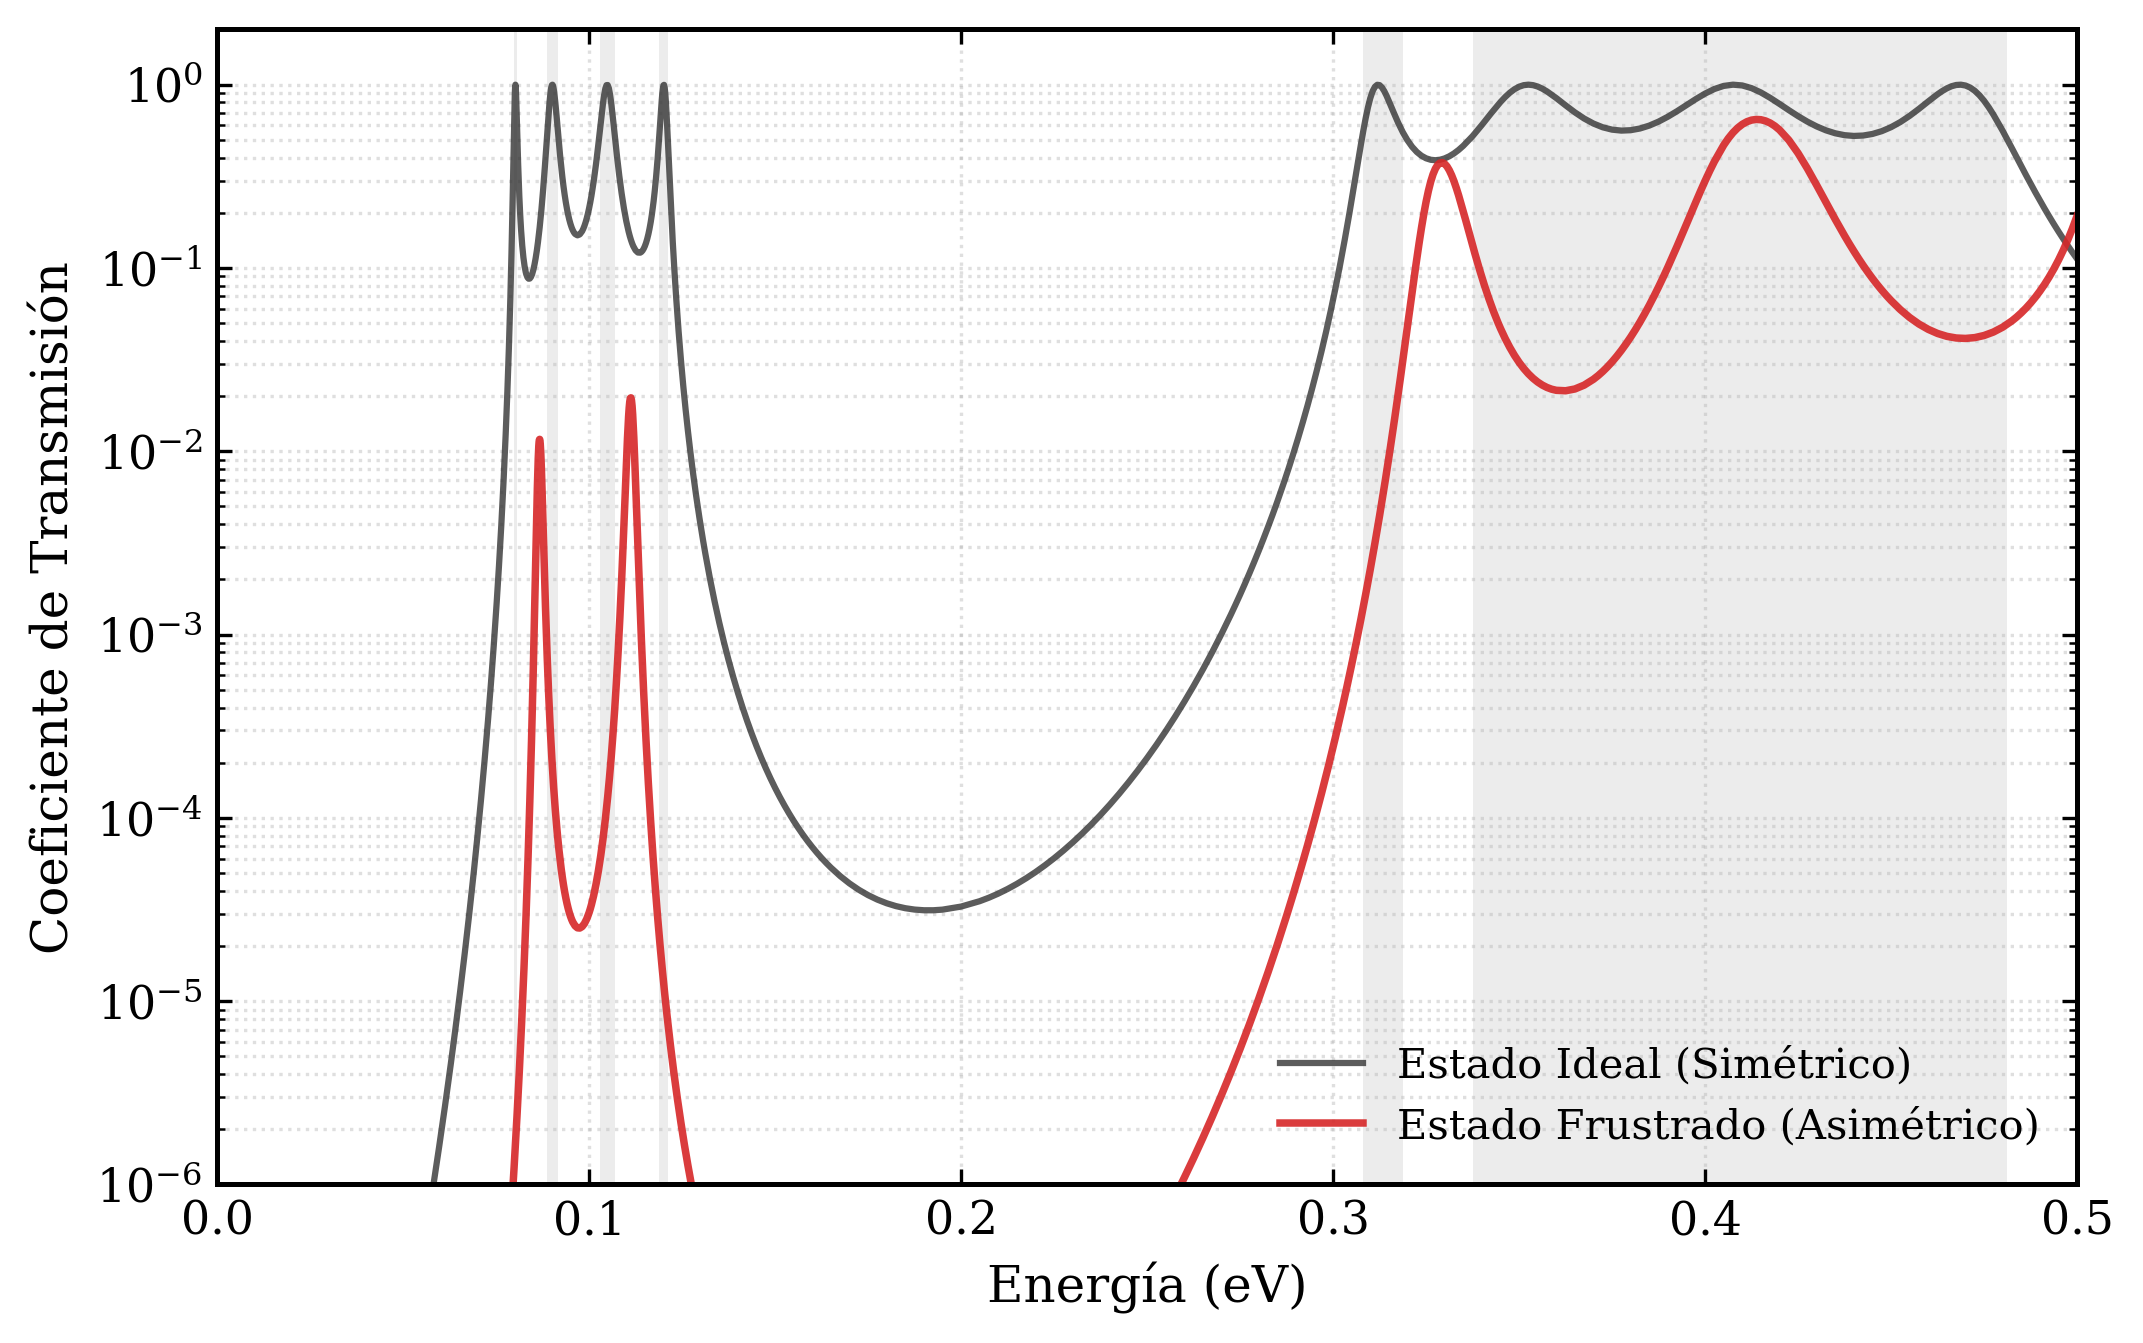
\includegraphics[width=1.0\linewidth]{Fig_Interfase_Rota.png}
  \caption{Efecto de la frustración por desalineación energética (célula mutada): Comparativa entre el filamento ideal (pozos simétricos de $6\text{ nm}$) y el filamento frustrado estructuralmente (pozo central ensanchado a $10\text{ nm}$).}
  \label{fig:Interfase_Rota}
\end{figure}

El segundo escenario simula una obstrucción física o calcificación en la interconexión celular central, incrementando la anchura de la barrera de potencial de $2\text{ nm}$ a $8\text{ nm}$. Los resultados de la Figura \ref{fig:Frustracion_Fuerte} muestran una atenuación de la transmitancia en todo el espectro energético analizado. 
A diferencia del caso anterior, aquí la frustración no se debe únicamente a un desajuste de niveles resonantes, sino a la dependencia matemática exponencial de la probabilidad de penetración de la barrera respecto a su espesor ($T \propto e^{-2\alpha w}$). Al cuadruplicar el espesor del septo la función de onda del electrón decae casi por completo en su interior, aislando eléctricamente ambas mitades de la hifa y anulando la capacidad de conducción del micelio.

\begin{figure}[H]
  \centering
  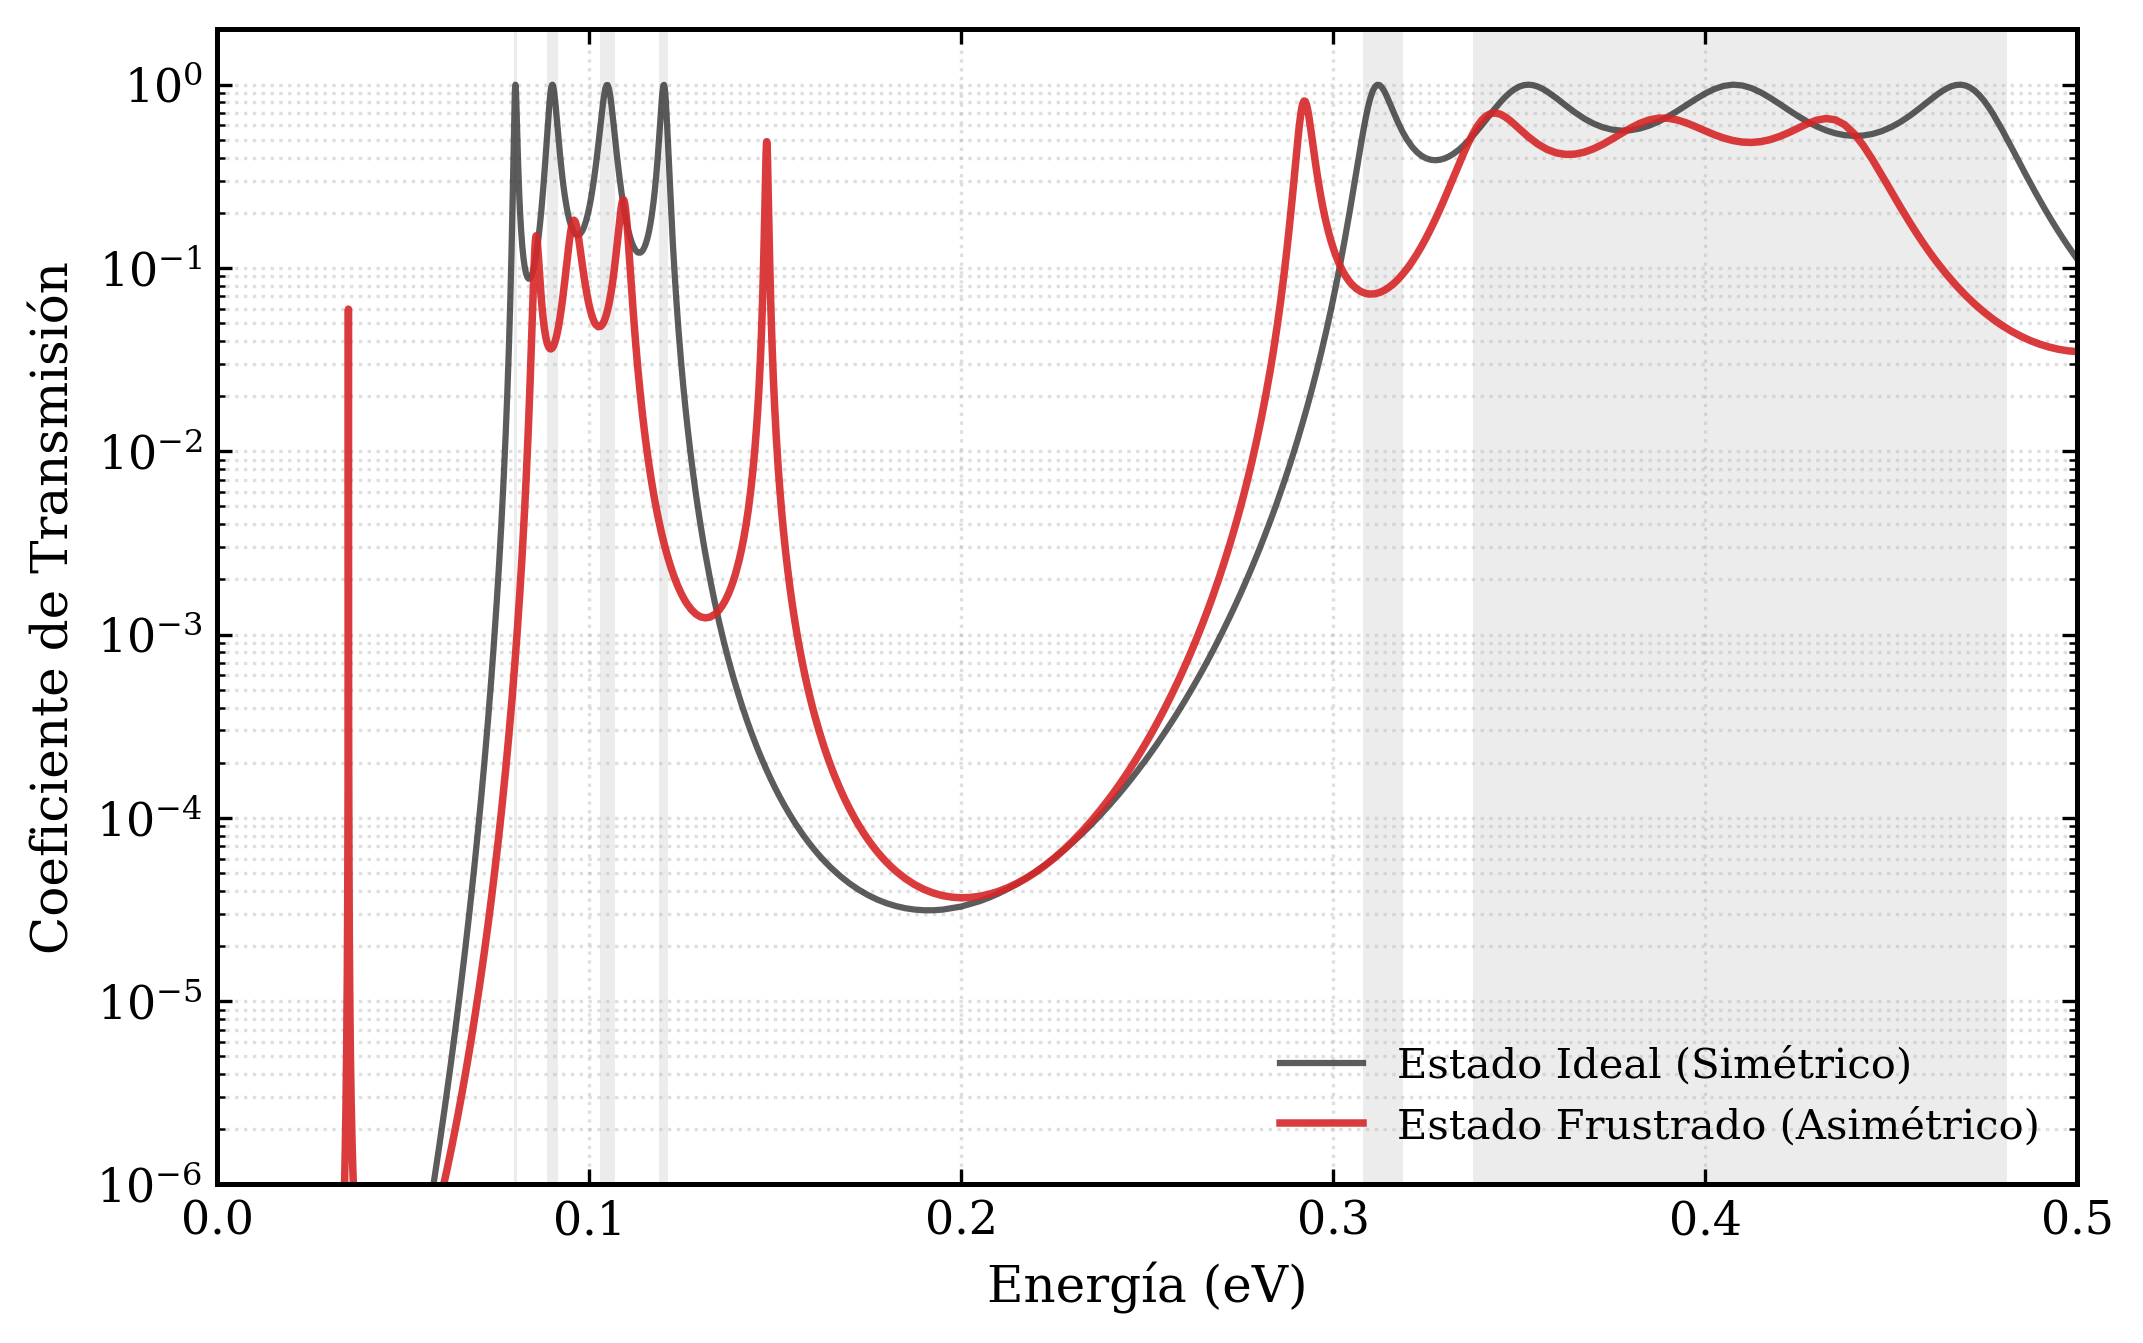
\includegraphics[width=1.0\linewidth]{Fig_Frustracion_Fuerte.png}
  \caption{Efecto de la frustración por bloqueo de interfase (septo calcificado): Respuesta del canal cuántico al aumentar el espesor de la barrera central de $2\text{ nm}$ a $8\text{ nm}$, evidenciando la disminución del coeficiente de transmisión.}
  \label{fig:Frustracion_Fuerte}
\end{figure}


\newpage
HOLA HOLA HOLA
\bibliographystyle{plain} 
\bibliography{refs}
\end{document}